\documentclass{article}

% PACKAGES for math, diagrams, and layout
\usepackage{amsmath}
\usepackage{amssymb}
\usepackage{tikz}
\usepackage{geometry}
\usepackage{graphicx} % Good practice to include for graphics

% DOCUMENT LAYOUT
\geometry{a4paper, margin=1in}

% --- DOCUMENT START ---
\begin{document}

\title{Two-Source Interference of Sound and Light Waves}
\author{Concise Notes for a 1-Hour Lesson}
\date{}
\maketitle

\section{The Core Principle: Superposition \& Coherence}

When two or more waves meet at a point, the resultant displacement is the vector sum of the individual displacements. This is the \textbf{principle of superposition}.

For interference to be observed, the sources must be \textbf{coherent}. This means they emit waves with a \textbf{constant phase difference} and the same frequency.

\begin{itemize}
    \item \textbf{Constructive Interference:} Waves arrive \textbf{in phase}. Crests meet crests. This results in a \textbf{maximum} amplitude (bright fringe for light, loud sound for audio).
    \item \textbf{Destructive Interference:} Waves arrive \textbf{out of phase} (by $180^\circ$ or $\pi$ radians). Crests meet troughs. This results in a \textbf{minimum} or zero amplitude (dark fringe for light, quiet spot for sound).
\end{itemize}

\begin{center}
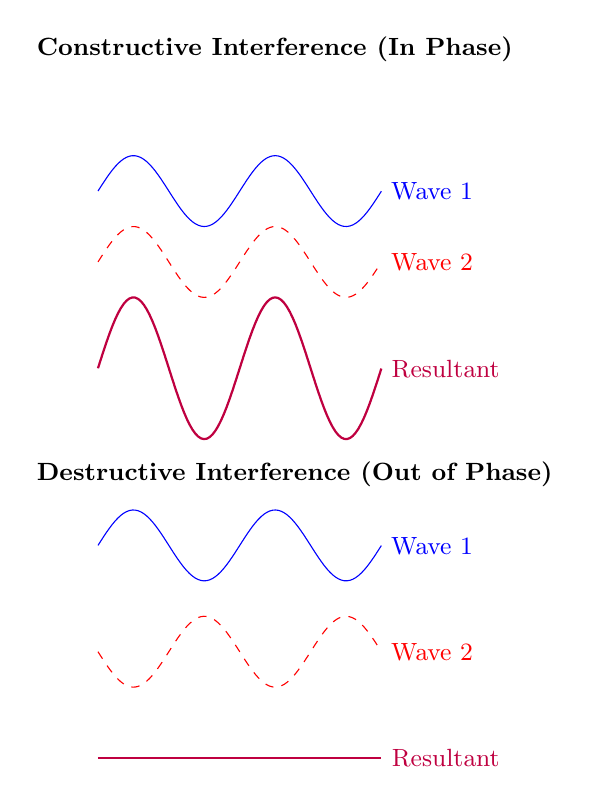
\begin{tikzpicture}[scale=0.9, every node/.style={font=\small}]
    % --- Constructive Interference ---
    \node[anchor=west] at (-1, 3) {\textbf{Constructive Interference (In Phase)}};
    % Wave 1
    \draw[blue, domain=0:4, samples=100] plot (\x, {1 + 0.5*sin(180*\x)}) node[right] {Wave 1};
    % Wave 2
    \draw[red, dashed, domain=0:4, samples=100] plot (\x, {0 + 0.5*sin(180*\x)}) node[right] {Wave 2};
    % Resultant
    \draw[purple, thick, domain=0:4, samples=100] plot (\x, {-1.5 + 1*sin(180*\x)}) node[right] {Resultant};

    % --- Destructive Interference (CORRECTED) ---
    \node[anchor=west] at (-1, -3) {\textbf{Destructive Interference (Out of Phase)}};
    % Wave 1
    \draw[blue, domain=0:4, samples=100] plot (\x, {-4 + 0.5*sin(180*\x)}) node[right] {Wave 1};
    % Wave 2 (This line is corrected to show proper phase inversion)
    \draw[red, dashed, domain=0:4, samples=100] plot (\x, {-5.5 - 0.5*sin(180*\x)}) node[right] {Wave 2};
    % Resultant (A flat line at zero amplitude)
    \draw[purple, thick] (0,-7) -- (4,-7) node[right] {Resultant};
\end{tikzpicture}
\end{center}

\hrulefill

\section{Path Difference: The Key to Interference}

The type of interference at a point depends on the \textbf{path difference} ($\Delta L$), which is the difference in the distance traveled by the two waves from their sources to that point.

\begin{center}
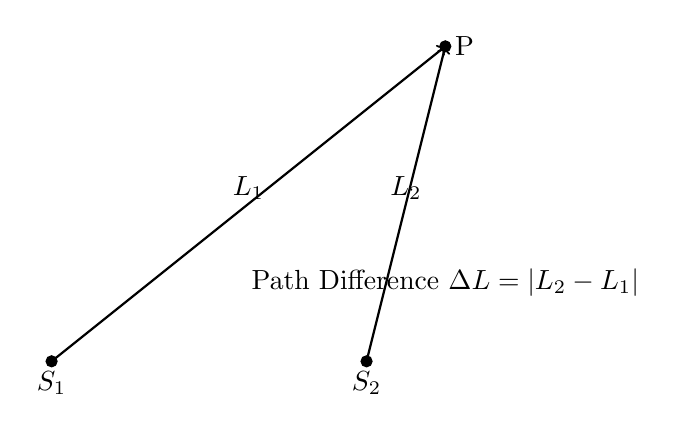
\begin{tikzpicture}
    \filldraw[black] (-2,0) circle (2pt) node[anchor=north] {$S_1$};
    \filldraw[black] (2,0) circle (2pt) node[anchor=north] {$S_2$};
    \filldraw[black] (3,4) circle (2pt) node[anchor=west] {P};
    \draw[->, thick] (-2,0) -- (3,4);
    \draw[->, thick] (2,0) -- (3,4);
    \node at (0.5,2.2) {$L_1$};
    \node at (2.5,2.2) {$L_2$};
    \node at (3, 1) {Path Difference $\Delta L = |L_2 - L_1|$};
\end{tikzpicture}
\end{center}

The path difference creates a \textbf{phase difference} ($\Delta \phi$). The relationship is:
\[
\Delta \phi = \frac{2\pi}{\lambda} \Delta L
\]

\subsection*{Conditions for Interference}
\begin{itemize}
    \item \textbf{Constructive Interference (Maxima):} \\
    The path difference is a whole number of wavelengths.
    \[
    \Delta L = n\lambda \quad \text{where } n = 0, 1, 2, ...
    \]
    \item \textbf{Destructive Interference (Minima):} \\
    The path difference is a half-integer number of wavelengths.
    \[
    \Delta L = \left(n + \frac{1}{2}\right)\lambda \quad \text{where } n = 0, 1, 2, ...
    \]
\end{itemize}

\hrulefill

\section{Application: Young's Double-Slit Experiment}

This setup demonstrates interference for both light and sound. The principles are identical.

\begin{center}
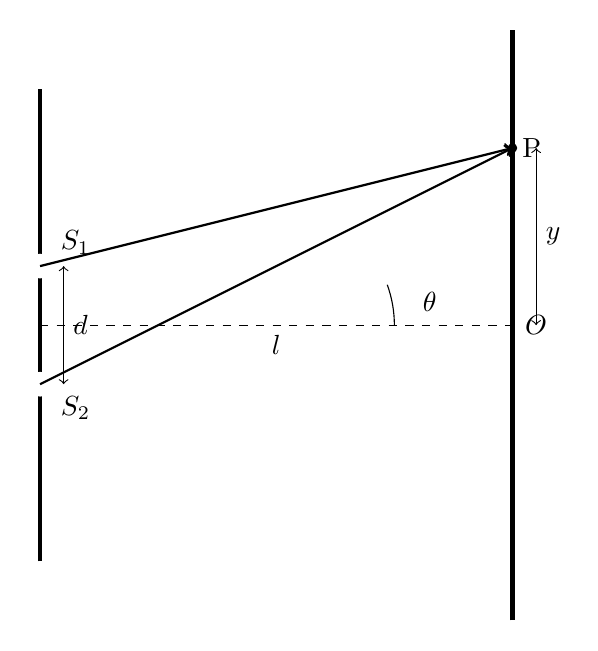
\begin{tikzpicture}[scale=1.5]
    % Slits
    \draw[ultra thick] (0,-2) -- (0,2);
    \filldraw[white] (0,0.5) circle (0.1);
    \filldraw[white] (0,-0.5) circle (0.1);
    \node at (0.3,0.7) {$S_1$};
    \node at (0.3,-0.7) {$S_2$};
    \draw[<->] (0.2,0.5) -- (0.2,-0.5) node[midway, right] {$d$};
    % Screen
    \draw[ultra thick] (4,-2.5) -- (4,2.5);
    \draw[dashed] (0,0) -- (4,0) node[midway, below] {$l$};
    \node at (4.2, 0) {$O$};
    % Point P
    \filldraw (4,1.5) circle (1pt) node[right] {P};
    \draw[<->] (4.2,0) -- (4.2,1.5) node[midway, right] {$y$};
    \draw[->, thick] (0,0.5) -- (4,1.5);
    \draw[->, thick] (0,-0.5) -- (4,1.5);
    % Angle theta
    \draw (3,0) arc (0:20:1);
    \node at (3.3, 0.2) {$\theta$};
\end{tikzpicture}
\end{center}

The path difference for rays traveling to point P is $\Delta L = d \sin \theta$. For a screen far away from the slits ($l \gg d$), we can find the position ($y$) of the fringes.

\newpage

\section{Advanced Topics & Problem-Solving Techniques}

\subsection{The Small Angle Approximation}
In many setups, the screen distance $l$ is much larger than the slit separation $d$ ($l \gg d$). This means the angle $\theta$ to any fringe is very small.
For small angles (in radians), we can approximate: $\sin\theta \approx \tan\theta$.
From the diagram, we see that $\tan\theta = y/l$.
So, the path difference becomes: $\Delta L = d \sin \theta \approx d \tan \theta = \frac{dy}{l}$.
\begin{itemize}
    \item For a bright fringe (maximum): $\frac{dy_n}{l} = n\lambda \implies y_n = \frac{n\lambda l}{d}$.
    \item The distance between adjacent bright fringes is:
    \[ \Delta y = y_{n+1} - y_n = \frac{(n+1)\lambda l}{d} - \frac{n\lambda l}{d} = \frac{\lambda l}{d} \]
\end{itemize}

\subsection{Intensity Distribution}
Let the waves from each slit have an amplitude $E_0$. The total electric field at a point on the screen is the superposition of two waves with a phase difference $\phi$:
\[ E = E_0\sin(\omega t) + E_0\sin(\omega t + \phi) \]
Using the identity $\sin\alpha+\sin\beta=2\cos\frac{1}{2}(\alpha-\beta)\sin\frac{1}{2}(\alpha+\beta)$:
\[ E = \left[ 2E_0 \cos\left(\frac{\phi}{2}\right) \right] \sin\left(\omega t + \frac{\phi}{2}\right) \]
The term in brackets is the new amplitude, $A = 2E_0 \cos(\phi/2)$. Intensity $I$ is proportional to the amplitude squared ($I \propto A^2$). If $I_0$ is the intensity from a single slit ($I_0 \propto E_0^2$), the resultant intensity is:
\[ I = 4I_0 \cos^2\left(\frac{\phi}{2}\right) = 4I_0 \cos^2\left(\frac{\pi d \sin\theta}{\lambda}\right) \]
The \textbf{maximum intensity} occurs when $\cos^2(\dots) = 1$, so $I_{max} = 4I_0$.

\subsection{Interference with Non-Normal Incidence}
What if the incoming light is not perpendicular to the slits, but arrives at an angle $\alpha$?
\begin{itemize}
    \item \textbf{Path difference before slits:} Before reaching the slits, one ray travels an extra distance compared to the other. This initial path difference is $\Delta L_{in} = d \sin \alpha$.
    \item \textbf{Path difference after slits:} As the rays leave towards the screen at an angle $\beta$, there is another path difference, $\Delta L_{out} = d \sin \beta$.
    \item \textbf{Total Path Difference:} The total path difference is the combination of these two effects. If the rays enter and leave on the \textbf{same side} of the normal, the total path difference is $\Delta L = |\Delta L_{in} - \Delta L_{out}| = |d(\sin\alpha - \sin\beta)|$. If they are on opposite sides, the path differences add.
    \item \textbf{Condition for Maxima:} For constructive interference, this total path difference must be an integer multiple of the wavelength.
    \[ |d(\sin\alpha - \sin\beta)| = n\lambda, \quad n=0, 1, 2, \dots \]
\end{itemize}

\subsection{Interference by Reflection (Lloyd's Mirror)}
This setup involves a direct wave and a reflected wave interfering (e.g., from a sound source S to a detector D).
\begin{itemize}
    \item The reflected path can be visualized as coming from a "virtual source" behind the reflector.
    \item \textbf{CRITICAL RULE:} Reflection from a denser medium (like sound in air hitting a solid wall) causes a $\boldsymbol{\pi}$ \textbf{radian ($180^\circ$) phase shift}.
    \item This phase shift is equivalent to adding an extra $\lambda/2$ to the geometric path length of the reflected wave.
    \item The conditions for interference are \textbf{swapped}:
        \begin{itemize}
            \item \textbf{Constructive (Loud/Bright):} Geometric path difference $\Delta L_{geo} = \left(n + \frac{1}{2}\right)\lambda$.
            \item \textbf{Destructive (Quiet/Dark):} Geometric path difference $\Delta L_{geo} = n\lambda$.
        \end{itemize}
    This is the key to solving problems like SPhO 2019 and 2023.
\end{itemize}

\hrulefill
\newpage

\section*{Competition Problems with Solutions}

\subsection{Problem 1 (SPhO 2024)}
\begin{quote}
Figure 10 shows an opaque screen in which there are two narrow parallel slits, P and Q, separated by a distance $d$. A beam of monochromatic light of wavelength $\lambda$ is incident on the screen at an angle $\alpha$ to the normal. Consider light emerging from the slits at an angle $\beta$ to the normal. Find an expression for the total path difference between rays 1 and 2 as a result of passing through the slits. Hence find the condition for the light emerging at angle $\beta$ to be of maximum intensity.
\end{quote}
\begin{center}
\begin{tikzpicture}[scale=1.2]
    % Slit screen
    \draw[ultra thick] (0,-1.5) -- (0,1.5);
    \node at (0,0.75) [label=left:P] (P) {};
    \node at (0,-0.75) [label=left:Q] (Q) {};
    \fill (P) circle (1.5pt);
    \fill (Q) circle (1.5pt);
    \draw[<->] (-0.2,0.75) -- (-0.2,-0.75) node[midway, left] {$d$};

    % Normal line
    \draw[dashed] (-2.5,0) -- (2.5,0);

    % Angle of incidence alpha (e.g., 30 degrees)
    \def\alpha{30}
    % Incoming parallel rays from top-right
    \draw[->, thick] (2, 0.75 - 2*tan(\alpha)) -- (P) node[pos=0.4, above, sloped] {Ray 1};
    \draw[->, thick] (2, -0.75 - 2*tan(\alpha)) -- (Q) node[pos=0.4, above, sloped] {Ray 2};

    % Angle alpha label
    \draw[->] (0.7,0) arc (0:-\alpha:-0.7);
    \node at (1.0, -0.25) {$\alpha$};

    % Angle of emergence beta (e.g., 20 degrees)
    \def\beta{20}
    % Outgoing rays to bottom-left
    \draw[->, thick] (P) -- ++(-180+\beta:2.5);
    \draw[->, thick] (Q) -- ++(-180+\beta:2.5);

    % Angle beta label
    \draw[->] (-0.7,0) arc (180:180-\beta:0.7);
    \node at (-1.0, 0.2) {$\beta$};

    \node at (0,-2) {Figure 10};
\end{tikzpicture}
\end{center}
\paragraph{Solution:}
\begin{enumerate}
    \item \textbf{Path difference before slits ($\Delta L_1$):} Before the slits, Ray 1 travels a longer path than Ray 2. This extra distance is $d \sin \alpha$.
    \item \textbf{Path difference after slits ($\Delta L_2$):} After the slits, Ray 2 travels a longer path than Ray 1. This extra distance is $d \sin \beta$.
    \item \textbf{Total path difference ($\Delta L_{\text{total}}$):} The net path difference is the absolute difference between these two values: $\Delta L_{\text{total}} = |d \sin \alpha - d \sin \beta|$.
    \item \textbf{Condition for maximum intensity:} For constructive interference (maximum intensity), the total path difference must be an integer multiple of the wavelength $\lambda$.
    \[ |d(\sin \alpha - \sin \beta)| = n\lambda, \quad \text{where } n = 0, 1, 2, ... \]
\end{enumerate}

\hrulefill

\subsection{Problem 2 (SPhO 2023) \& 4 (SPhO 2019)}
\begin{quote}
A sound source S and a detector D are placed 120 m apart. The source produces sound with wavelength 1.33 m. A reflector is parallel to the line SD. At position 1 (90 m from SD), the direct wave is in phase with the reflected wave. The reflector is moved away to position 2.
\begin{itemize}
    \item \textbf{2023 Problem:} At position 2, intensity is zero for the first time. Find $h$.
    \item \textbf{2019 Problem:} At position 2, intensity is maximum again for the first time. Find $h$.
\end{itemize}
\end{quote}
\begin{center}
\begin{tikzpicture}
    \node at (0,0) [circle,fill,inner sep=1pt,label=above:S] {};
    \node at (8,0) [circle,fill,inner sep=1pt,label=above:D] {};
    \draw[<->] (0,-0.2) -- (8,-0.2) node[midway, below] {120 m};
    % Reflector
    \draw[thick] (0,3) -- (8,3) node[midway, label={[label distance=0.1cm]90:Reflector}] {};
    \node at (9,3) {Position 1};
    \draw[thick, dashed] (0,4) -- (8,4) node[midway, above] {};
    \node at (9,4) {Position 2};
    % Distances
    \draw[<->] (9.5,3) -- (9.5,4) node[midway, right] {$h$};
    \draw[<->] (8.2,0) -- (8.2,3) node[midway, right] {90 m};
    \node at (4,-0.75) {Fig. 1};
\end{tikzpicture}
\end{center}
\paragraph{Solution:}
Let $L=120$ m and $y$ be the reflector distance. Path difference $\Delta L_{geo} = 2 \sqrt{y^2 + (L/2)^2} - L$.
\begin{enumerate}
    \item \textbf{Condition at Position 1:} At $y_1 = 90$ m, waves are in phase (constructive). With a $\pi$ phase shift on reflection, the condition is $\Delta L_{geo} = (m+1/2)\lambda$.
    $\Delta L_1 = 2 \sqrt{90^2 + 60^2} - 120 = 96.33$ m.
    $m + 1/2 = 96.33/1.33 = 72.43 \implies m=72$.

    \item \textbf{For SPhO 2023 (First Minimum):} The next fringe is destructive, where $\Delta L_{geo} = k\lambda$. The next order is $k=73$.
    $\Delta L_2 = 73 \times 1.33 = 97.09$ m.
    $2 \sqrt{y_2^2 + 60^2} - 120 = 97.09 \implies y_2 = 90.45$ m.
    $h = y_2 - y_1 = 90.45 - 90 = \textbf{0.45 m}$.

    \item \textbf{For SPhO 2019 (Next Maximum):} The next fringe is constructive, corresponding to $m=73$.
    $\Delta L_2 = (73 + 1/2)\lambda = 73.5 \times 1.33 = 97.755$ m.
    $2 \sqrt{y_2^2 + 60^2} - 120 = 97.755 \implies y_2 = 90.85$ m.
    $h = y_2 - y_1 = 90.85 - 90 = \textbf{0.85 m}$.
\end{enumerate}

\hrulefill

\subsection{Problem 3 (SPhO 2021)}
\begin{quote}
Consider Young's double slit experiment. (a) Under what condition does it show an interference pattern? (b) Determine the conditions for constructive and destructive interference. (c) Determine the distance $\Delta y$ between adjacent fringes, assuming $\theta$ is small. (d) Determine the intensity I of the diffraction pattern's maxima.
\end{quote}
\begin{center}
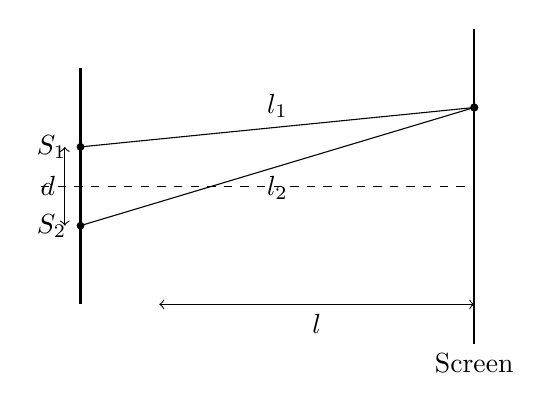
\begin{tikzpicture}
    % Slits
    \draw[thick] (0,1.5) -- (0,-1.5);
    \node at (0,0.5) [circle,fill,inner sep=1pt,label=left:$S_1$] {};
    \node at (0,-0.5) [circle,fill,inner sep=1pt,label=left:$S_2$] {};
    \draw[<->] (-0.2,0.5) -- (-0.2,-0.5) node[midway, left] {$d$};
    % Screen
    \draw[thick] (5,2) -- (5,-2) node[below] {Screen};
    % Paths
    \draw (0,0.5) -- (5,1) node[midway,above] {$l_1$};
    \draw (0,-0.5) -- (5,1) node[midway,below] {$l_2$};
    \fill (5,1) circle (1.5pt);
    % Center line
    \draw[dashed] (-0.5,0) -- (5,0);
    % Labels
    \draw[<->] (1,-1.5) -- (5,-1.5) node[midway,below] {$l$};
\end{tikzpicture}
\end{center}
\paragraph{Solution:}
\begin{itemize}
    \item[(a)] The light from the two slits must be \textbf{coherent}.
    \item[(b)] Path difference $\Delta L = d \sin \theta$.
        \begin{itemize}
            \item \textbf{Constructive:} $d \sin \theta = n\lambda$.
            \item \textbf{Destructive:} $d \sin \theta = (n+1/2)\lambda$.
        \end{itemize}
    \item[(c)] Using small angle approx, $\sin\theta \approx y/l$. Position of $n$-th max is $y_n = n\lambda l/d$.
    The distance between adjacent fringes is $\Delta y = y_{n+1} - y_n = \frac{\lambda l}{d}$.
    \item[(d)] The intensity is $I = 4I_0 \cos^2(\frac{\phi}{2})$, where $I_0$ is the intensity of a single slit and $\phi$ is the phase difference. The maximum intensity $I_{max}$ occurs when the cosine-squared term is 1, so $I_{max} = \textbf{4I}_0$.
\end{itemize}

\end{document}
% --- DOCUMENT END ---